%%%%%%%%%%%%%%%%%%%%%%%%%%%%%%%%%%%%%%%%%%%%%%%%%%%%%%%%%%%%%%%%%%%%%%%%%%%%%
% SP Communication Core Documentation
% ----------------------------
% Last Updated: February 18, 2013
%
% To change the configuration of the code scripts, change the settings 
% in the CODE CONFIGURATION section. 
%
%%%%%%%%%%%%%%%%%%%%%%%%%%%%%%%%%%%%%%%%%%%%%%%%%%%%%%%%%%%%%%%%%%%%%%%%%%%%%

%----------------------------------------------------------------------------------------
%	PACKAGES AND OTHER DOCUMENT CONFIGURATIONS
%----------------------------------------------------------------------------------------

\documentclass{article}

\usepackage{fancyhdr} 					% Custom headers
\usepackage{lastpage} 					% To determine the last page for the footer
\usepackage{extramarks} 				% Headers and footers
\usepackage[usenames,dvipsnames]{color} 		% Custom colors
\usepackage{graphicx} 					% Insert images
\usepackage{listings} 					% Insertion of code
\usepackage{courier} 					% Courier font
\usepackage{lipsum}
\usepackage{longtable}
\usepackage{color}

% Margins
\topmargin=-0.45in
\evensidemargin=0in
\oddsidemargin=0in
\textwidth=6.5in
\textheight=9.0in
\headsep=0.25in

\linespread{1.1} % Line spacing

%----------------------------------------------------------------------------------------
%	CODE CONFIGURATION
%----------------------------------------------------------------------------------------

\definecolor{MyDarkGreen}{rgb}{0.0,0.4,0.0} % Color used for block comments
\definecolor{MyRed}{rgb}{0.6,0,0}% Color used for strings
\definecolor{MyPurple}{rgb}{0.5,0,0.35} % keywords
\definecolor{MyBlue}{rgb}{0.25,0.35,0.75} % more comment
\definecolor{HighlighterYellow}{rgb}{1,1,0}% highlighter color to indicate changed lines

\newcommand{\Highlight}{\makebox[0pt][1]{\color{HighlighterYellow}\rule[-4pt]{0.65\linewidth}{14pt}}}

\lstloadlanguages{C} 						% Load C syntax for listings, for a list of other languages supported see: ftp://ftp.tex.ac.uk/tex-archive/macros/latex/contrib/listings/listings.pdf

\lstset{
	language=C,
	keywordstyle=\color{MyPurple},
	stringstyle=\color{MyRed},
	commentstyle=\color{MyDarkGreen},
	morecomment=[s][\color{MyBlue}]{/**}{*/},
	numbers=left,
	numbersep=5pt,
	tabsize=4,
	showspaces=false,
	showstringspaces=false,
	breaklines=true,
	basicstyle=\footnotesize,
	title=\lstname
}

% Creates a new command to include a C script, the first parameter is the filename of the script (without .c), the second parameter is the caption
\newcommand{\cscript}[2]{
\begin{itemize}
\item[]\lstinputlisting[caption=#2,label=#1]{#1.c}
\end{itemize}
}

%----------------------------------------------------------------------------------------
%   OTHER DOCUMENT CONFIGURATIONS
%----------------------------------------------------------------------------------------

% Auto-incremented caption labels
\newcommand{\cscriptcode}[2]{
\begin{itemize}
\item[]\lstinputlisting[caption=#2,label=#1]{#1.c}
\end{itemize}
}

%----------------------------------------------------------------------------------------
%	AUTHOR AND OTHER DOCUMENT INFORMATION 
%----------------------------------------------------------------------------------------

\newcommand{\docTitle}{Manual}					           % Documentation title
\newcommand{\lastUpdate}{April 2nd,\ 2014} 			% Last updated
\newcommand{\projectTitle}{CP/SP Communication and Organization}	% Project title
\newcommand{\institution}{Northern Arizona University\\Wireless Networks Research Laboratory} 	% Institution
\newcommand{\authorNames}{Michael Middleton} 	% Authors
\newcommand{\location}{Flagstaff,\ AZ}					% Location

% Project description
\newcommand{\projectDescription}{This document discusses the developments and discoveries regarding serial communication between CP and SP boards following the latest revision.}	


%----------------------------------------------------------------------------------------
%	HEADER AND FOOTER 
%----------------------------------------------------------------------------------------
\pagestyle{fancy}
%\lhead{\lastUpdate} 						% Top left header
\rhead{\projectTitle:\ \docTitle} 					% Top center head
%\lhead{\firstxmark} 						% Top right header
\lfoot{\lastxmark} 							% Bottom left footer
\cfoot{} 									% Bottom center footer
\rfoot{Page\ \thepage\ of\ \protect\pageref{LastPage}} 	% Bottom right footer
\renewcommand\headrulewidth{0.4pt} 			% Size of the header rule
\renewcommand\footrulewidth{0.4pt} 			% Size of the footer rule

\setlength\parindent{0pt} % Removes all indentation from paragraphs

%----------------------------------------------------------------------------------------
%	TITLE PAGE
%----------------------------------------------------------------------------------------

\newcommand*{\titleGroup}
{\begingroup % Create the command for including the title page in the document
	\centering % Center all text
	\vspace*{\baselineskip} % White space at the top of the page
	\vspace*{10pt}

	\rule{\textwidth}{1.6pt}\vspace*{-\baselineskip}\vspace*{2pt} 	% Thick horizontal line
	\rule{\textwidth}{0.4pt}\\[\baselineskip] 				% Thin horizontal line

	{\LARGE \projectTitle}\\[0.2\baselineskip]	 			% Title

	\rule{\textwidth}{0.4pt}\vspace*{-\baselineskip}\vspace{3.2pt} 	% Thin horizontal line
	\rule{\textwidth}{1.6pt}\\[\baselineskip] 				% Thick horizontal line

	\scshape % Small caps
	\projectDescription \\[\baselineskip] 	% Tagline(s) or further description
	\location\par 				% Location
	\lastUpdate\par 			% Last updated 

	\vspace*{2\baselineskip} % Whitespace between location/year and editors

	Edited by \\[\baselineskip]
	{\Large \authorNames\par} 	% Author list
	{\itshape \institution\par} % Author affiliation

	\vfill % Whitespace between editor names and publisher logo

\endgroup}

%----------------------------------------------------------------------------------------

\begin{document}

\thispagestyle{empty}
\titleGroup


%----------------------------------------------------------------------------------------
%	TABLE OF CONTENTS
%----------------------------------------------------------------------------------------

%\setcounter{tocdepth}{1} % Uncomment this line if you don't want subsections listed

\newpage
\tableofcontents
\newpage

%----------------------------------------------------------------------------------------
%	OVERVIEW
%----------------------------------------------------------------------------------------

\section{Overview}
An investigation of the WiSARD UART communication implementation has yielded performance information regarding the accuracy and precision of data sampling and has provided new insight into the limitations of the maximum baud rate possible on current WiSARD hardware. The previous revision of the UART communication implementation between CP and SP contained undesirable latencies in the transmission and sampling of serial messages due to an approach that was functional but was not optimal for fast and efficient communication.
\\\\
New revisions to the communication code involving the restructuring of the Port2 and Timer0 A0 interrupt service routines and the behavior of functions within the protocol have allowed for a communication system that is resilient to errors and mis-sampling, as well as an overall improved form which utilizes good software engineering practices and robust design. Figure 1 shows the sampling of a single byte from a command packet sent from CP to an SP light board. The activity represented by the light blue is the CP transmit line and the yellow activity is a trace that depicts the time at which the SP samples the line. The rising and falling edges of the trace indicate the precise moment that the code enters the switch-case statement to processes the current bit, located in the receiveByte function (Appendix B.1,  line 339).  

\begin{figure}[!h]
\centerline{\includegraphics[scale=0.5]{9600_Byte_CPtoSP}}
\caption{CP to SP byte transmission}
\end{figure}

Figure 2 depicts the transmission and sampling of an entire 32-bit message from the same command packet as Figure 1. These images show an overall improvement in sampling accuracy and precision over the previous revision of the communication code. On average, samples are taken within 1us of the middle of every bit across all baud rates, whereas the code from the previous revision would often be within 2us of the center of a bit.

\begin{figure}[!h]
\centerline{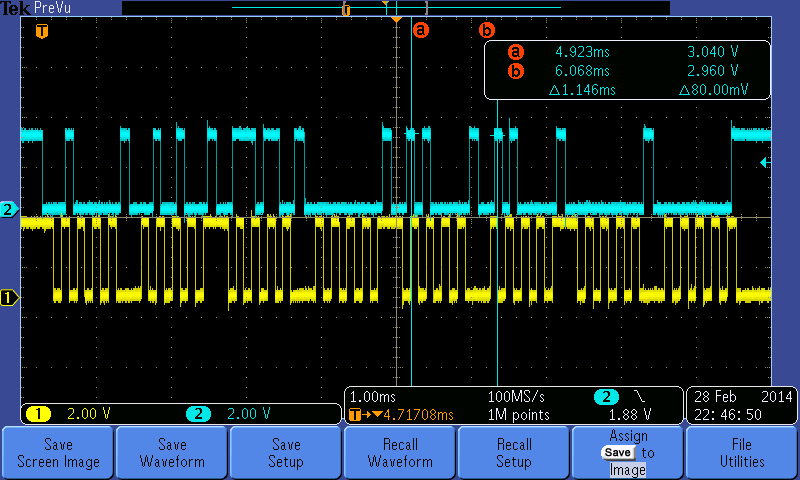
\includegraphics[scale=0.5]{9600_PACKET_CPtoSP}}
\caption{CP to SP 32-bit packet transmission}
\end{figure}

%----------------------------------------------------------------------------------------
%	CODE REORGANIZATION
%----------------------------------------------------------------------------------------
\newpage
\section{Code Reorganization}
The previous revision of the UART communication implementation between CP and SP contained latencies from a few different sources, most significantly from the Timer0 A0 interrupt service routine. Other latencies and behavioral issues in the communication code developed from the manner in which data messages were received within the Timer0 A0 ISR, the mishandling of the wake up times, and the lack of a consistent generalized approach to sampling in the center of each bit.   

\subsection{Interrupt Service Routines}
Timer0 A0 uses a 4MHz SMCLK to count up to the length of a single bit, defined by the current baud rate, and then triggers a Timer0 A0 interrupt. In the transmission code, when the Timer0 A0 interrupt is triggered, the TX line will be pulled high or low depending upon the value of the next bit in the message to be sent. The receiver portion uses the same interrupt to sample the TX line, determine the location of the bit in the message, and shift the bit to its correct location in the received message on the RX buffer. Previously, the code within the ISR contained the logic used to determine whether the hardware was sending or receiving a message, and then handled the message bit appropriately (Appendix A.3). Even though the bits were being handled as soon as the interrupt was triggered, issues arose from executing this logic within the ISR. At the time the interrupt is triggered, the timer is halted and execution moves to the code within in the ISR. The 2.5us time associated with waking the MCU from LPM0 and sequentially evaluating the message logic effectively stalls the start of Timer0 A0 counting to the next bit until execution returns from the ISR. This approach to sending and receiving messages is problematic because the time required to execute the ISR compounds with each bit of a transmitted byte. Note that TX and RX re-synchronize at each byte with the falling edge of the start bit.
\\\\
To remedy the negative effects of structuring the code in this manner, a new approach was developed which reorganized the way in which the code was executed. The first step was to remove the message logic from the Timer0 A0 ISRs and place them into sendByte() and receiveByte() functions. These functions would be called once for each byte transmission or reception and rest in LPM0 while waiting for the next bit to be sent or received. The sole operation of the Timer0 A0 ISR, now that the message logic has been removed, is to simply wake the MCU from LPM0 and return to program execution (Appendix A.4). The ISR no longer needs to check the state of the hardware either, since the waking from LPM0 is required whether the hardware is in transmission or reception. This change exhibits good form within interrupt driven design as the ISRs are as simple as possible, and make the smallest impact on the continuity between hardware components. Additionally, these changes make the code more modular in its design. Byte transmission and reception, as well as waking from LPM0 are now decoupled and can be altered independent of the other components. This will help in making future edits and revisions simpler to debug and easier to navigate.

\subsection{Generalized Delay Solution}
Further changes made to the communication code involved mitigating delays associated with a receiver sampling the first data bit of a byte. Following the falling edge of the TX-line, which indicates the start of a byte transmission, the receiver would ideally wait the duration of the start bit, and half the duration of a second bit so that the first sample will be taken in the middle of the data bits. This leaves the largest possible error tolerance. In the previous revision, each baud rate used a hard-coded number of clock cycles on the 4MHz SMCLK to indicate approximately one half of the bit length respectively (Appendix B.2). There was no uniformity to the way in which these values were achieved and they did not completely account for the full wake up time from LPM3 when sampling the first byte of a new packet. The time required to wake from LPM3 as listed in the MSP430x5xx family users guide is approximately 9us.
\\\\
To handle this problem with a more generalized solution, a single formula was used to calculate the delay values and account for the 9us wake up time for LPM3. By implementing the formula [(1.5 * BaudRateControl) - 36] clock cycles calculated for a 4MHz SMCLK, a generalized delay for the sampling as well as compensating for MCU wake up time was achieved across the baud rates 115200, 57600, 19200, and 9600 (Appendix B.3). This formula is generalized such that it can be used to calculate the half bit delay for any baud rate with Timer0 A0 sourced from a 4MHz SMCLK. This formula works because the 36 clock cycles at 4MHz accounts for the same 9us delay present regardless of the current baud rate.

%----------------------------------------------------------------------------------------
%	FASTER BAUD RATES
%----------------------------------------------------------------------------------------
\section{Faster Baud Rates}
Current WiSARD hardware supports the possibility of baud rates faster than 115200, though doing so would require a new approach to sending and receiving messages. The current approach places the MCU in LPM0 while Timer0 A0 counts on the appropriate interval. Waking the MCU from LPM0 takes 2.5us, regardless of baud rate. The baud rate 230400 is such that the length of a single bit is 4.34us. The LPM0 wakeup time is greater than the half bit delay required for 230400 at the start of each byte. Accommodating the half bit delay would require that for a baud rate of 230400, the MCU would need to remain on for the duration of the message on both the transmission and reception. Additionally, the 9us delay necessary to wake the MCU from LPM3 would require transmitters to send packets with multiple exceptionally long start bits, thus breaking compliance with the protocol specification. Specifically, the length of the start bit is adequate to accommodate the wakeup time for all baud rates up to 115200 but 230400 would need at least 9us, which would require slightly longer than 2 start bits. Adding additional bits to the front of a packet would mean that the communication is no longer within the formal specification of the UART protocol, meaning that interfacing with third party hardware or software which communicates via UART would no longer be a possibility. Since 115200 is the fastest baud rate incorporating low power modes while maintaining UART communication specifications, the decision was made to forsake the implementation of faster baud rates for the time being.
\\\\

%----------------------------------------------------------------------------------------
%	CP Code
%----------------------------------------------------------------------------------------
\newpage
\appendix
\section{CP Code Modifications}

	\subsection{SP.c (Current Revision)}
This function contains the majority of the logic for byte transmission that was removed from the Timer0 A0 interrupt service routine.
	\lstinputlisting[
		title = SendByte Function,
		firstline  = 560, 
		lastline = 656,
		firstnumber = 560
		]{listings/CP/SP.c}

This function contains the majority of the logic for byte reception that was removed from the Timer0 A0 interrupt service routine.
	\lstinputlisting[
		title = ReceiveByte Function,
		firstline = 656,
		lastline = 778,
		firstnumber = 656
	]{listings/CP/SP.c}

This function contains the logic necessary for the receiver to adapt its anticipated message size based upon the packet header which it receives.
	\lstinputlisting[
		title = WaitForMessage Function,
		firstline = 838, 
		lastline = 876,
		firstnumber = 838
		]{listings/CP/SP.c}

	\subsection{SP.h (Current Revision)}
The following code demonstrates the current definitions for the baud rate delay values which utilizes the generalized delay cycle calculation formula.
	\lstinputlisting[
		firstline = 349, 
		lastline = 360,
		firstnumber = 349
		]{listings/CP/SP.h}

	\subsection{irupt.c (Previous Revision)}	
The following code demonstrates the previous behavior of the Timer0 A0 interrupt service routine.
	\lstinputlisting[
		firstline = 250,
		lastline = 313,
		firstnumber = 250
		]{listings/CP/old_irupt.c}

	\subsection{irupt.c (Current Revision)}
The following code demonstrates the current behavior of the Timer0 A0 interrupt service routine.
	\lstinputlisting[
		firstline = 237, 
		lastline = 244,
		firstnumber = 237
		]{listings/CP/irupt.c}


%----------------------------------------------------------------------------------------
%	 SP Code
%----------------------------------------------------------------------------------------
\newpage
\section{SP Code Modifications}
	\subsection{comm.c (Current Revision)}
This function contains the majority of the logic for byte transmission that was removed from the Timer A0 interrupt service routine.
	\lstinputlisting[
		title = SendByte Function,
		firstline = 227, 
		lastline = 299,
		firstnumber = 227
		]{listings/SP/comm.c}

	\lstinputlisting[
		title = receiveByte Function,
		firstline = 301,
		lastline = 402,
		firstnumber = 301
		]{listings/SP/comm.c}

	\subsection{comm.c (Current Revision)}
The following code provides the reduced Timer0 A0 interrupt service routine which handles the waking of the MCU from LPM0.
	\lstinputlisting[
		title = Timer0 A0 ISR,
		firstline = 683, 
		lastline = 692,
		firstnumber = 683
		]{listings/SP/comm.c}

	\subsection{comm.h (Previous Revision)}
This following code demonstrates the hard-coded definitions for the baud rate delay values. 
	\lstinputlisting[
		firstline = 96,
		lastline = 107,
		firstnumber = 96
		]{listings/SP/old_comm.h}

	\subsection{comm.h (Current Revision)}
The following code demonstrates the current definitions for the baud rate delay values which utilizes the generalized delay cycle calculation formula.
	\lstinputlisting[
		firstline = 97, 
		lastline = 110,
		firstnumber = 97
		]{listings/SP/comm.h}

%----------------------------------------------------------------------------------------

\end{document}